\chapter{Assessing Cyber Power}

After exploring the concepts essential to develop a coherent approach for our analysis, this section will delve into assessing cyber power and the different methods and theoretical frameworks that the academic literature presents.  At a crossroads in the age of digital revolution, the European Union is debating whether or not to be taken seriously as a major actor in the internet arena. On a global scale, the idea of cyber power, which includes the capacity to exercise influence, control, and shaping over events in the digital sphere, is becoming more and more prominent. The academic community is finding that the existing corpus of information is fragmented and frequently overshadowed by the dominance of the United States' vision as it attempts to understand the complex relationship between cyber capabilities and global power dynamics.

While scholars and practitioners have extensively debated the concept of power in international relations over the centuries, the nature of power in the digital age presents unique challenges and opportunities. Traditional realist perspectives view power primarily as a tool of coercion, emphasizing military and economic strength. However, in cyberspace, the dynamics of power extend beyond brute force, encompassing elements such as information control, technological proficiency, and the ability to shape public opinion and narratives.

As the European Union expands its international influence in various domains, including international trade and human rights, its foray into the realm of cybersecurity and foreign policy appears less pronounced. The EU's unique character and political structure make it challenging to assess its role as a cyber power. Does the European Union utilize cyberspace to gain advantages and project influence on a global scale, transcending traditional notions of state security? While sovereign states primarily bear the responsibility for securing cyberspace, the EU's approach to cybersecurity charts new paths that extend beyond conventional understandings of power.

Measuring cyber power is a formidable undertaking, complicated by the lack of standardised methods and frameworks for assessment. Cyberspace's distinct characteristics, including its layered structure and the secrecy surrounding many cyber capabilities, further compound the challenge. In response to this complex landscape, this chapter delves into the intricacies of assessing cyber power, exploring various models and indices that attempt to shed light on the European Union's role in the digital arena.

By examining models such as Nye's Three Faces Model, Klimburg's Power Integrated Capability Model, and Betz and Stevens' Four Dimension Model, this chapter seeks to unravel the multifaceted nature of cyber power. These models offer different perspectives on power, encompassing coercion, institutional influence, structural change, and the construction of social subjects through discourse. By scrutinising these models, we aim to discern the EU's capacity to wield power in cyberspace and its unique approach, which leans towards cooperation rather than coercion.

The concept of power has been debated and studied for centuries, with scholars and practitioners recognising its central role in international relations. Power is essential to achieving goals and maintaining influence in the international realm \autocite{holsti_1964_the}. Realist scholars have particularly emphasised power as a key variable in international politics, defining the study of international relations in terms of power, and viewing it as the currency of great-power politics \autocite{fels_2016_power}. According to Morgenthau, power in international relations is a central concept and the main objective of a nation's foreign policy. He defined power as the ability to maintain and increase a nation's power while reducing the power of other nations \autocite{morgenthau_1948_politics}. 

Constructivist scholars have challenged the realist concept of power in the realm of complex interdependence in the international system. According to \textcite{pan_2014_rethinking}, power is a social construct instead of a concept that is quantitatively measurable and has a zero-sum property. \textit{Power is multifaceted, and the different facets come with strengths and weaknesses that are context- and issue-dependent} \autocite[14]{dunncavelty_2018_europes}. The perception of power is even more important in cyberspace because it shapes the dynamics and implications of power within the cyberspace domain. In this context, it is not exclusively decided by economic or military strength but also by elements such as information control, technological proficiency, and the capacity to affect public opinion and build narratives.

Barnett and Duvall \textcite{barnett_2005_power} presented a more contemporary understanding of power, proposing a taxonomic framework to categorise power concepts. They identified four distinct concepts of it:

\begin{enumerate}
    \item \textbf{Compulsory power}: one actor exerts control over another to make them do something they would not otherwise choose to do. This power is typically exercised through direct coercion, such as the use of force or threats.
    \item \textbf{Institutional power}: This form of power operates through the creation and maintenance of institutions that shape and influence the behaviour of actors. These institutions can take various forms, ranging from formal organisations to informal social structures. Both state and non-state actors can create this.
    \item \textbf{Structural power}: This type of power is exerted through the establishment and maintenance of social structures that shape the behaviour of actors. These structures may be of an economic, political, or cultural nature, and both state and non-state actors may be responsible for their creation. Structural power operates by influencing the opportunities and constraints that individuals and groups encounter in these social systems.
    \item \textbf{Productive power}: This form of power operates through the production of subjects through diffuse social relationships. It shapes actors’ capacities to define their circumstances and determine their own destinies through the creation and dissemination of norms, values, and identities.
\end{enumerate}
        

\section{How to assess Cyber Power?}

The most well-known index related to cyberspace is the \textit{Global Cybersecurity Index} (GCI), launched in 2015 by the \textit{International Telecommunication Union} (ITU). The aim of the index is to measure ITU Member States’ commitment to cybersecurity. The CGI focuses on legal, technical, organizational, capacity development, and cooperation areas to evaluate each country \autocite{internationaltelecommunicationunion_2020_global}. However, the military and defence sectors are not involved because the objective of the International Organization is to technically evaluate the cybersecurity aspects. This study is based on a multi-stakeholder approach and involves countries that cooperate and promote knowledge exchange in the sector. However, due to its nature, the organisation was not able to verify all the collected data because several countries denied it \autocite[viii]{internationaltelecommunicationunion_2020_global}. 

A recent study conducted by the \textit{Belfer Center for Science and International Affairs} at Harvard Kennedy School, known as the \textit{National Cyber Power Index}, sought to measure cyber power. This study, initially published in 2020 and subsequently updated in 2022, takes a comprehensive approach to assess both potential and demonstrated cyber capabilities. The index focuses on scoring each country based on a range of objectives, including surveillance and monitoring domestic groups, strengthening national cyber defences, controlling and manipulating the information environment, foreign intelligence collection for national security, growing national cyber and commercial technology competence, destroying or disabling an adversary's infrastructure and capabilities, defining international cyber norms and technical standards, and amassing wealth and/or extracting cryptocurrency \autocite[5-6]{voo_2022_national}. These objectives directly or indirectly contribute to a state's overall capability, allowing scholars to assess them beyond mere rhetoric and in conjunction with other tools used to achieve national interests, such as military or diplomatic means \autocite{voo_2022_national}.  


The \textit{Cyber Arms Watch} and its \textit{Cyber Transparency Index}, developed by The Hague Centre for Strategic Studies, is another index that analyses the transparency of a state's cyber offensive capabilities. It focuses on measuring difficult-to-assess aspects of transparency. The index incorporates the \textit{Declared Capabilities Rating} (DCR), which assesses the extent to which a state publicly discloses information about its offensive cyber capability. This includes official government communications and authorised media reports, which are classified using a six-tiered labelling system. The classification ranges from no official indication of offensive cyber capabilities to various levels of disclosure. Additionally, Cyber Arms Watch introduces the \textit{Perceived Capabilities Rating} (PCR), which evaluates the perceived offensive cyber capabilities of a state based on open-source information. This rating uses external sources such as intelligence reports, assessments from other governments or non-state actors, indictments, sanctions, past operations, and leaked documents. PCR employs the same six-level categorisation system to classify the observed capabilities of a state as perceived by outsiders \autocite[4]{faesen_2022_cyber}. The computed \textit{Cyber Transparency Index}, a difference between the \textit{PCR} and \textit{DCR}, is calculated to create clusters of cyber transparency for the 60 countries analysed. In Figure \ref{fig:cybercap}, the European countries and the biggest international actors are displayed. 

It is evident that identifying countries that demonstrate transparency regarding their cyber capabilities is a challenging task, not only within nations characterised by low levels of democracy but also within the European Union. The lack of disclosure concerning cyber strategies presents a significant obstacle to future research in this field. However, this study highlights a clear pattern: nations frequently overestimate their cyber capabilities. Additionally, the difficulties in accurately assessing actual cyber offensive capabilities are further compounded by attribution. States frequently use hacktivist groups or other entities as fronts for their operations in cyberspace, making it difficult to identify the specific state that is accountable.

Research has become increasingly challenging when considering the specific cyber capabilities possessed by the EU. To delve deeper into this matter, this study comprehensively examines and compares the cyber capabilities of Member States with those of the EU.

\begin{figure}[H]
    \centering
    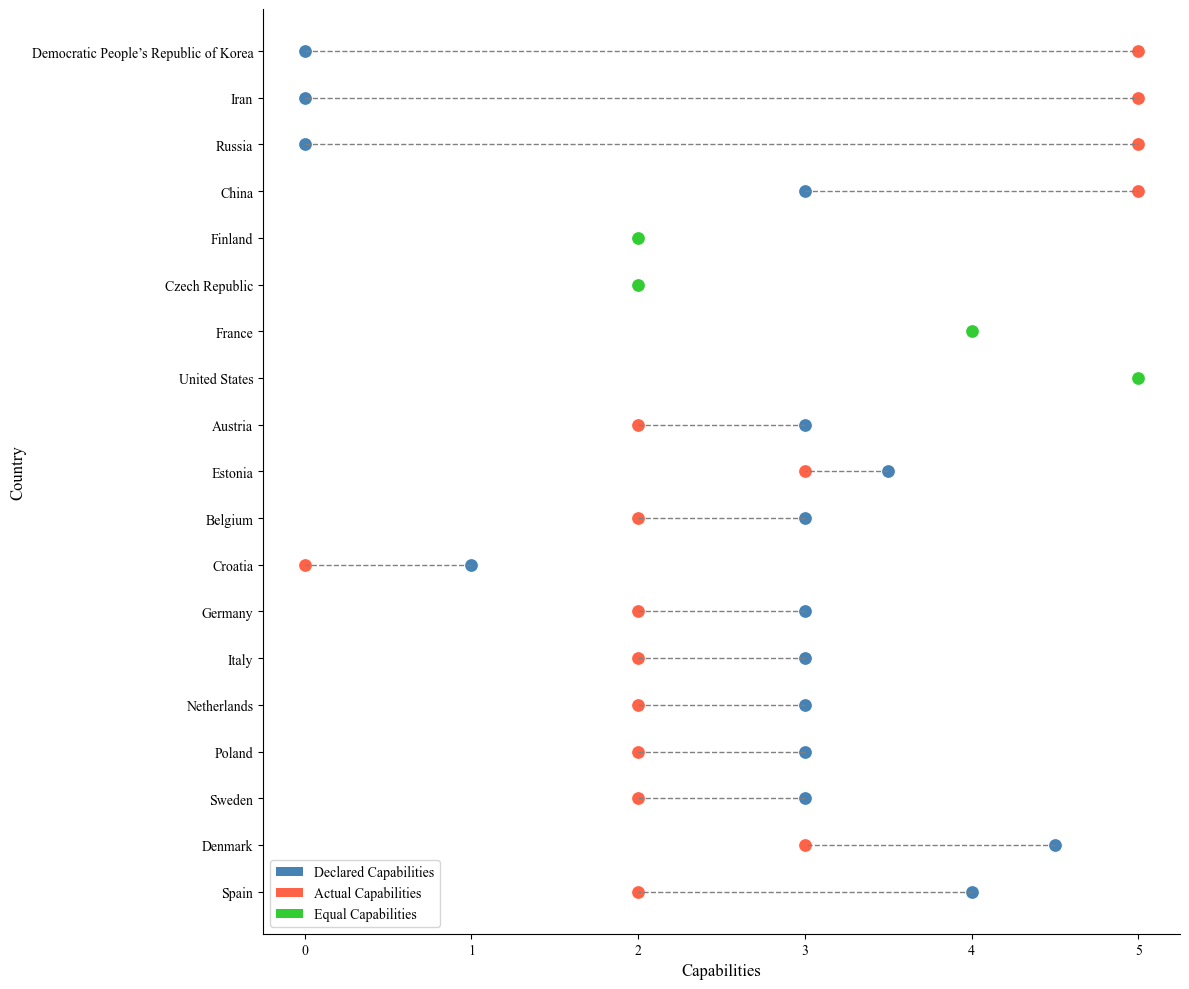
\includegraphics[width=1\textwidth]{Images/cybercap.png}
    \caption{\textit{Cyber Transparency Index \autocite[4]{faesen_2022_cyber}}}
    \label{fig:cybercap}
\end{figure}

Several analytical frameworks have been developed to assess the cyber power of a state. Each model focuses on a different approach to the power concept. In this analysis, we examine Nye’s \textit{Three Faces Model } \autocite{nye_2010_cyber}, the\textit{ Klimburg’s Power Integrated Capability Model} \autocite{klimburg_2011_cybersecurity} and the \textit{Betz and Stevens Four Dimension Model} \autocite{betz_2011_cyberspace}. All the models present power as a form of domination, in contrast to power as empowerment, \parencite{haugaard_2012_rethinking, dunncavelty_2018_europes} with the expectation of Klimburg.

According to Nye  \textcite{nye_2010_cyber}, both hard and soft power can be used to achieve political goals in cyberspace. His “Three Faces Model” identifies three types of power relations, that are not exclusively adopted only in the cyber environment between two different actors (A and B in this case). Nye identified the specific means and methods with an effect in cyberspace, which constitute power \autocite{vanhaaster_2016_assessing}). 

\begin{enumerate}

   \item The 1st face refers to the capacity of an actor (A) to force another actor (B) to engage in actions that they would not have taken otherwise. The author investigated the utilisation of malware or other attack vectors, such as DDoS attacks, to disrupt critical national services and coerce B to take measures to counter the attack. 
   \item The 2nd face involves A’s strategies to block B’s actions. Chinese “Great Firewall” is an empirical example. Nye referred to this as an agenda-setting power.
   \item The 3rd face refers to A’s power to influence B’s preferences. The author uses the example of threats to punish bloggers who disseminate censored material as preventive actions to shape their preferences.
\end{enumerate}

\begin{table}[htbp]
  \centering
  \caption{\emph{Three Faces Model of Cyberpower according to Nye \textcite{nye_2010_cyber}}}
  \begin{tabular}{p{4cm}p{4.5cm}p{5.5cm}}
    \toprule
    \textbf{Type of Power} & 
    \textbf{Hard Power} 
            (Nye) & 
    \textbf{Soft Power} 
            (EU's case) \\
    \midrule
    1st Face (A induces B to do what B would initially otherwise not do) & 
    \begin{itemize}
      \item Denial of Service attacks
      \item Insertion of malware
      \item Scada disruptions
      \item Arrests of bloggers
    \end{itemize} &
    \begin{itemize}
      \item Cybersecurity Act
      \item Mutual Defense Clause: Art. 42(7) of the TUE
      \item Cyber Diplomacy Toolbox for diplomatic retaliation
      \item NIS 1 \& 2
      \item European Cyber Defence Policy
    \end{itemize} \\
    \midrule
    2nd Face (A precludes B’s choice by the exclusion of B’s strategies) &
    \begin{itemize}
      \item Firewalls, filters, and pressure on companies to exclude some ideas
    \end{itemize} &
    \begin{itemize}
      \item Budapest Convention
      \item European Chips Act
    \end{itemize} \\
    \midrule
    3rd Face (A shapes B’s preferences so some strategies are never even considered) &
    \begin{itemize}
      \item Threats to punish bloggers who disseminated censored material
    \end{itemize} &
    \begin{itemize}
      \item General Data Protection Regulation (GDPR)
      \item AI Act
    \end{itemize} \\
    \bottomrule
  \end{tabular}
  
\raggedright
    \bigskip
    Source: Elaboration from Dunn Cavelty \textcite[11]{dunncavelty_2018_europes} (author’s example).
\end{table}



Nye’s model implies that cyber capabilities can produce both hard and soft powers \autocite[5]{nye_2010_cyber}. In this regard, the European Union, unlike Nye’s examples, does not have the hard power capabilities to achieve political objectives for each of the faces. However, EU legislation gives us the opportunity to assess EU cyper power through legislative acts, which lie more as soft power instruments rather than harder ones. Furthermore, the distinction between hard and soft cyberspace is difficult \autocite[5]{dunncavelty_2018_europes}. 

Nye suggests that cyber capacities are widespread, with all actors capable of conducting diverse cyber activities, such as denial-of-service attacks, issuing threats, controlling information, and suppressing ideas. This widespread nature casts doubt on its effectiveness as an independent analytical tool for policymakers, despite its significance in academia \autocite{vanhaaster_2016_assessing}.


\begin{table}[htbp]
  \caption{\emph{Klimburg Power Integrated Capability Model}}
  \begin{tabular}{p{7cm}p{7cm}}
    \toprule
    \textbf{Type of Power} & \textbf{Definition} \\
    \midrule
    Integrated Government Capability & Ability to deliver joint action \\
    \midrule
    Integrated Systems Capability & Ability to work through international alliances and partnerships \\
    \midrule
    Integrated National Capability & Ability to use non-state cyber elements within a country in direct support of policy \\
    \bottomrule
  \end{tabular}
  
    \raggedright
        \bigskip
    Source: Elaboration from \textcite[12]{dunncavelty_2018_europes}.
\end{table}

The Klimburg Power Integrated Capability Model understands cyber power in terms of integrated capabilities, which can shape the cybersecurity landscape \parencite{kasper_2021_the, klimburg_2011_cybersecurity}. According to \textcite{klimburg_2011_mobilising}, cyber power is the result of distributed forces. His model includes several dimensions, such as the ability to coordinate government actions, collaborate with international partners, and engage with non-state actors (both businesses and hacktivists) \parencite{dunncavelty_2018_europes, klimburg_2011_cybersecurity}. The model implies a more defensive posture of cyber power rather than an offensive character aimed at coercing other actors. The concept of cyber resilience, which has become increasingly relevant in Europe, stems from this model. As \textcite[6]{dunncavelty_2018_europes} stated, \textit{there cannot be any true cyber-power without cyber-resilience.}

A common critique is related to the EU, which according to several scholars \parencite{kasper_2021_the, klimburg_2011_cybersecurity, sliwinski_2014_moving}, does not have sufficient cyber power. This is because, by embedding the realist assumptions of state power, scholars give more importance to the 1st face or more simply to the military side of power, which creates difficulties for the EU due to the characteristics of its political project and the uncertainty in assessing cyber capabilities \autocite{dunncavelty_2018_europes}. However, the EU is more focused on cyber power based on cooperation instead of coercion because of its nature and scope, which highlights the main difference between the EU and other organisations such as NATO. 

Authors such as \textcite{kasper_2021_the} further explored the Klimburg Power Integrated Capability Model by adding a new layer that pertains to the strategic narratives of European cyber power. The authors stated that the EU has not yet been able to formulate a strategic identity narrative while opting for a non-military approach regarding its international approach to cybersecurity \autocite[64]{kasper_2021_the}. Indeed, the EU's involvement in international forums and conferences and the continuous growth of its cyber capabilities, which extend beyond securing the digital market, serve as examples of its increasing cyber power. Doubts remain regarding the hard cyber power capabilities of the union. 

The \textcite{betz_2011_cyberspace} model effectively applies \textcite{barnett_2005_power} power taxonomy to the realm of cyberspace, providing a distinct categorisation of power manifestations within this domain. This model introduces an additional layer to the Three Faces of Power model by adopting a post-structuralist approach, perceiving power as circulating within social relationships \autocite{dunncavelty_2018_europes}. 

\begin{table}[htbp]
  \centering
  \caption{\emph{Betz and Stevens (2011) Cyber Power Taxonomy}}
  \begin{tabularx}{\textwidth}{p{4cm}p{5cm}p{5cm}}
    \toprule
    \textbf{Type of Power} & \textbf{Definition} & \textbf{Examples} \\
    \midrule
    Compulsory & Coercion to change the behaviour of another actor & Control of machines or networks \\
     & Deploying non-material resources & \\
    \midrule
    Institutional & Indirect control of another actor through institutions & Influence behaviour through institutions \\
     & Norms and Standards & \\
    \midrule
    Structural & Cyberspace as a structure which can facilitate or disrupt the actors that are connected & Changing structures \\
    \midrule
    Productive & Creation of social subjects through discourse & Reproduce, construct, and reinforce narratives \\
    \bottomrule
  \end{tabularx}
  
  \raggedright
  \bigskip
  Source: Elaboration from \textcite{betz_2011_cyberspace} and \textcite{dunncavelty_2018_europes} .
\end{table}

The model identifies four distinct types of power in the cyberspace context \parencite{betz_2011_cyberspace, dunncavelty_2018_europes, vanhaaster_2016_assessing}:

\begin{enumerate}
    \item \textbf{Compulsory Power}: This type of power involves the use of coercion to compel another actor to change its behaviour. It can be exerted through the control of machines or networks, as well as through the deployment of non-material resources. For instance, a state may use cyber-attacks to disrupt the operations of an adversary or hacktivists may employ cyber means to force a corporation to change its policies.
    \item \textbf{Institutional Power}: In category, power is exercised indirectly through institutions. Actors may influence the behaviour of others through the establishment and manipulation of norms, standards, and protocols in cyberspace. Governments and international organisations, for example, can shape behaviour through the creation of cybersecurity regulations and standards that impact the actions of various actors in the digital realm.
    \item \textbf{Structural Power}: This type of power acknowledges cyberspace as a structure that can either facilitate or disrupt the actors connected to it. Actors may wield power by altering or controlling the underlying structure of cyberspace. For instance, a powerful tech company might shape the architecture of the Internet or a state might exert control over the global routing of data to enhance its strategic advantage.
    \item \textbf{Productive Power}: Productive power in cyberspace refers to the creation of social subjects through discourse. This involves shaping and influencing narratives, constructing ideologies, and reinforcing certain beliefs and values in the digital space. Governments, media organisations, and influential online communities may engage in shaping public opinion and generating narratives that support their interests.
\end{enumerate}

Conversely, the Klimburg and Nye models suggest that cyber capabilities can be utilised within a specific domain or context. Alternatively, Betz and Stevens adopted a post-structuralist perspective on cyber power \autocite{dunncavelty_2018_europes}, emphasising the location of the conflict rather than solely on the cyber capabilities deployed \autocite{vanhaaster_2016_assessing}. All cyber tools have the potential to be employed to achieve various state objectives, whether they are related to military, political, or economic power. \textcite[21]{vanhaaster_2016_assessing} argues that \textit{it is impossible to create a comprehensive overview of cyber power distribution, as it relies on all dimensions of power}. Because these dimensions are contextual and some are temporary, the field should refrain from adopting a universal model for assessing cyber power and instead employ frameworks on a case-by-case basis. 

In conclusion, \textcite{vanhaaster_2016_assessing} builds a cyber capacity framework on the state’s instruments of power as described by various authors and frameworks, namely Carr, Mann, and DIME(FIL) proponents.  These scholars have expounded on how these instruments can be effectively employed to exert influence in traditional domains such as land, sea, and air. The model in question seeks to expand this discussion into the realm of cyberspace and identify the cyber analogues of these instruments of state power. This endeavour holds significant importance given the prevailing cyber power discourse's tendency to predominantly focus on the means aspect of power, such as the capacity for conducting \textit{Distributed Denial of Service} (DDoS) attacks and the allocation of budgets for acquiring malware. Nevertheless, this viewpoint falls short of encompassing a myriad of factors that collectively contribute to a state's capacity to achieve its objectives in cyberspace. This study presents a more comprehensive and holistic approach to analysing cyber power by identifying and understanding the cyber equivalents of traditional instruments of state power. This inclusive approach incorporates consideration of factors such as the extent of influence, the specific domain of operation, the magnitude of impact, associated costs, and the means employed, each of which plays a vital role in comprehending a state's true capability to wield power in the digital arena. 

\begin{table}[htbp]
  \centering
  \caption{\emph{State's Power Instruments and Cyber Capacities according to \textcite{vanhaaster_2016_assessing}}}
  \begin{tabularx}{\textwidth}{p{2.5cm}X}
    \toprule
    \textbf{Instrument} & \textbf{Cyber Capacities} \\
    \midrule
    \multirow{2}{*}{Political} & Coordination \\
    & Cyber-capacities to be used abroad \\
    & Deterrence \\
    \midrule
    \multirow{2}{*}{Informational} & Manipulation of information \\
    & Legitimization through social media \\
    & Intelligence gathering \\
    \midrule
    \multirow{2}{*}{Economical} & Protect own industries \\
    & Secure infrastructure \\
    \midrule
    \multirow{2}{*}{Military} & Kinetic-Cyber coordination \\
    & Military infrastructure control \\
    \midrule
    Other & Influence institutions \\
    & Arrests or prosecuting \\
    & International Law applied to cyber \\
    \bottomrule
  \end{tabularx}
  \label{tab:state-power-cyber}
\end{table}


\newpage

The framework serves as a foundational point for analysing cyber strategies, considering five essential dimensions that warrant a thorough case-by-case assessment:
\begin{itemize}
 \item \textbf{Scope}: This dimension encompasses the extent of cyber power, the number of actors involved, and the geographic area covered.
 \item \textbf{Domain}: Here, the focus lies on the specific areas or sectors where cyber power is wielded, be it in the military, economic, or political domains.
 \item \textbf{Weight}: This dimension evaluates the relative importance or significance of cyber power in comparison with other forms of power at play.
 \item \textbf{Costs}: The resources necessary to develop and sustain cyber power are scrutinized by incorporating financial, human, and technological resources.
 \item \textbf{Means}: Finally, attention is paid to the specific tools, techniques, and capabilities employed to exercise and manifest cyber power.
\end{itemize}

Considering these five dimensions, the framework provides a comprehensive and multifaceted approach to the analysis of cyber power strategies, thereby offering valuable insights into the dynamics and effectiveness of such endeavours. This framework will be applied in the analysis of the cyber realm of the War in Ukraine to retrieve key lessons for other actors. 


